\chapter{Kubus dan Balok}\label{ch:g5:solids}

Meninggalkan halaman yang datar: \omterm{def:g5:solids:def}{bangun ruang} adalah bentuk dunia
nyata --- dadu, kotak sereal, kaleng, bola. Bab ini belajar
menamainya, membilang sisi dan \omterm{def:g5:solids:def}{rusuknya}, membukanya menjadi
\omterm{def:g5:solids:net}{jaring-jaring}, lalu mengukur \omterm{def:g5:solids:volume}{volumenya} dengan membilang \omterm{def:g5:solids:def}{kubus} kecil.
(Rumus \omterm{def:g5:solids:volume}{volume} menyusul pada \cref{ch:g6:measure}.)

\section{Keluarga bangun ruang}

\begin{definition}[Bangun ruang dan kosakatanya]\label{def:g5:solids:def}
\emph{Bangun ruang}\index{bangun ruang} menempati ruang. Bidang
datarnya disebut \emph{sisi}\index{sisi}; sisi bertemu sepanjang
\emph{rusuk}\index{rusuk}; rusuk bertemu di \emph{titik
sudut}\index{titik sudut}. Potret keluarganya:
\begin{itemize}
  \item \emph{kubus}\index{kubus}: $6$ sisi berbentuk persegi, $12$
        rusuk, $8$ titik sudut;
  \item \emph{balok}\index{balok} (prisma persegi panjang): $6$ sisi
        berbentuk persegi panjang, $12$ rusuk, $8$ titik sudut;
  \item \emph{tabung}\index{tabung}: dua sisi berbentuk cakram dan satu sisi
        yang tergulung (sebuah kaleng);
  \item \emph{limas}\index{limas}: alas berbentuk \omterm{def:g4:geometry:polygon}{segi banyak} dan segitiga yang
        bertemu di satu puncak;
  \item \emph{bola}: satu permukaan bundar sempurna, tanpa sisi
        datar dan tanpa rusuk.
\end{itemize}
\end{definition}

\begin{omfigure}
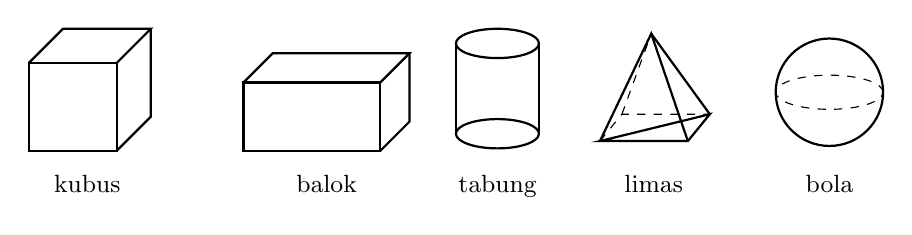
\begin{tikzpicture}[scale=0.62]
  % kubus
  \draw[thick] (0,0) rectangle (1.8,1.8);
  \draw[thick] (0,1.8) -- (0.7,2.5) -- (2.5,2.5) -- (1.8,1.8);
  \draw[thick] (2.5,2.5) -- (2.5,0.7) -- (1.8,0);
  \node[below, font=\small] at (1.2,-0.3) {kubus};
  % balok
  \begin{scope}[xshift=4.4cm]
  \draw[thick] (0,0) rectangle (2.8,1.4);
  \draw[thick] (0,1.4) -- (0.6,2.0) -- (3.4,2.0) -- (2.8,1.4);
  \draw[thick] (3.4,2.0) -- (3.4,0.6) -- (2.8,0);
  \node[below, font=\small] at (1.7,-0.3) {balok};
  \end{scope}
  % tabung
  \begin{scope}[xshift=9.6cm]
  \draw[thick] (0,0.35) ellipse (0.85 and 0.3);
  \draw[thick] (-0.85,0.35) -- (-0.85,2.2);
  \draw[thick] (0.85,0.35) -- (0.85,2.2);
  \draw[thick] (0,2.2) ellipse (0.85 and 0.3);
  \node[below, font=\small] at (0,-0.3) {tabung};
  \end{scope}
  % limas
  \begin{scope}[xshift=12.6cm]
  \draw[thick] (-0.9,0.2) -- (0.9,0.2) -- (1.35,0.75) -- cycle;
  \draw[thick] (-0.9,0.2) -- (0.15,2.4) -- (0.9,0.2);
  \draw[thick] (1.35,0.75) -- (0.15,2.4);
  \draw[dashed] (-0.9,0.2) -- (-0.45,0.75) -- (1.35,0.75);
  \draw[dashed] (-0.45,0.75) -- (0.15,2.4);
  \node[below, font=\small] at (0.2,-0.3) {limas};
  \end{scope}
  % bola
  \begin{scope}[xshift=16.4cm]
  \draw[thick] (0,1.2) circle (1.1);
  \draw[dashed] (0,1.2) ellipse (1.1 and 0.35);
  \node[below, font=\small] at (0,-0.3) {bola};
  \end{scope}
\end{tikzpicture}

{\small Galeri \omterm{def:g5:solids:def}{bangun ruang}. Garis putus-putus menunjukkan \omterm{def:g5:solids:def}{rusuk}
yang tersembunyi --- bagian belakang bangun itu, dilihat menembusnya.}
\end{omfigure}

\begin{example}[Membilang pada kubus]\label{ex:g5:solids:count}
Periksalah pada sebuah dadu: $6$ sisi (bilangan $1$ sampai $6$), $8$
\omterm{def:g5:solids:def}{titik sudut} (pojoknya), $12$ \omterm{def:g5:solids:def}{rusuk} (rabalah dengan jari: $4$ di
atas, $4$ di bawah, $4$ tegak). Dan $6 + 8 = 12 + 2$ --- pola aneh
yang sama juga berlaku untuk \omterm{def:g5:solids:def}{balok} dan \omterm{def:g5:solids:def}{limas}
(\cref{ex:g8:solids:count} kembali membahasnya).
\end{example}

\section{Jaring-jaring}

\begin{definition}[Jaring-jaring]\label{def:g5:solids:net}
\emph{Jaring-jaring}\index{jaring-jaring} sebuah \omterm{def:g5:solids:def}{bangun ruang} adalah
gambar datar semua sisinya, yang tersambung sepanjang \omterm{def:g5:solids:def}{rusuk}, dan
yang terlipat menjadi \omterm{def:g5:solids:def}{bangun ruang} itu --- \omterm{def:g5:solids:def}{bangun ruang} yang dibuka
seperti kardus yang dipipihkan untuk didaur ulang.
\end{definition}

\begin{omfigure}
\begin{tikzpicture}[scale=0.5]
  \draw[gray!40, thin] (0,0) grid (4,3);
  \draw[thick, omDef] (0,1) rectangle (1,2);
  \draw[thick, omDef] (1,1) rectangle (2,2);
  \draw[thick, omDef] (2,1) rectangle (3,2);
  \draw[thick, omDef] (3,1) rectangle (4,2);
  \draw[thick, omDef] (1,2) rectangle (2,3);
  \draw[thick, omDef] (1,0) rectangle (2,1);
  \node[below, font=\small] at (2,-0.5) {sebuah jaring-jaring kubus};
  \begin{scope}[xshift=7.5cm]
  \draw[gray!40, thin] (0,0) grid (4,3);
  \draw[thick, omThm] (0,1) rectangle (1,2);
  \draw[thick, omThm] (1,1) rectangle (2,2);
  \draw[thick, omThm] (2,1) rectangle (3,2);
  \draw[thick, omThm] (3,1) rectangle (4,2);
  \draw[thick, omThm] (0,2) rectangle (1,3);
  \draw[thick, omThm] (0,0) rectangle (1,1);
  \node[below, font=\small] at (2,-0.5) {jaring-jaring lain yang sah};
  \end{scope}
  \begin{scope}[xshift=15cm]
  \draw[gray!40, thin] (0,0) grid (4,3);
  \draw[thick, omExo] (0,1) rectangle (1,2);
  \draw[thick, omExo] (1,1) rectangle (2,2);
  \draw[thick, omExo] (2,1) rectangle (3,2);
  \draw[thick, omExo] (3,1) rectangle (4,2);
  \draw[thick, omExo] (0,2) rectangle (1,3);
  \draw[thick, omExo] (1,2) rectangle (2,3);
  \node[below, font=\small] at (2,-0.5) {bukan jaring-jaring! (mengapa?)};
  \end{scope}
\end{tikzpicture}

{\small Tiga susunan enam persegi. Dua yang pertama terlipat menjadi
\omterm{def:g5:solids:def}{kubus}; yang ketiga tidak --- ketika dilipat, dua persegi mendarat di
sisi yang sama dan kubusnya tetap terbuka. Guntinglah lalu cobalah!}
\end{omfigure}

\begin{example}[Membaca jaring-jaring]\label{ex:g5:solids:read}
Pada sebuah dadu, sisi yang berhadapan berjumlah $7$. Pada
\omterm{def:g5:solids:net}{jaring-jaring}, sisi yang berhadapan adalah yang terpisah tepat satu
persegi dalam satu baris (atau memutari pojok) --- bukan
tetangganya! Menandai pasangannya pada \omterm{def:g5:solids:net}{jaring-jaring} sebelum melipat
adalah latihan yang bagus untuk melihat ruang secara datar.
\end{example}

\section{Volume: membilang kubus}

\begin{definition}[Volume dengan membilang]\label{def:g5:solids:volume}
\emph{Volume}\index{volume} sebuah \omterm{def:g5:solids:def}{bangun ruang} yang dibangun dari
\omterm{def:g5:solids:def}{kubus} satuan adalah banyaknya \omterm{def:g5:solids:def}{kubus} yang dimuatnya. Satuannya bisa
\omterm{def:g5:solids:def}{kubus} sentimeter (cm$^3$) atau \omterm{def:g5:solids:def}{kubus} meter (m$^3$).
\end{definition}

\begin{example}[Membilang balok lapis demi lapis]\label{ex:g5:solids:layers}
Sebuah \omterm{def:g5:solids:def}{balok} sepanjang $4$ \omterm{def:g5:solids:def}{kubus}, selebar $3$, setinggi $2$: lapisan
dasarnya memuat $4 \times 3 = 12$ \omterm{def:g5:solids:def}{kubus}, dan ada $2$ lapisan:
\[
12 \times 2 = 24 \text{ kubus} .
\]
Membilang per lapisan selalu berhasil --- dan diam-diam ia
membuktikan rumus $V = L \times w \times h$ pada \cref{ch:g6:measure}.
\end{example}

\begin{omfigure}
\begin{tikzpicture}[scale=0.52]
  \foreach \y in {0,1} {
    \foreach \x in {0,...,3} {
      \foreach \z in {0,1,2} {
        \begin{scope}[shift={({\x+0.4*\z},{\y+0.28*\z})}]
          \draw[fill=omDef!12] (0,0) rectangle (1,1);
          \draw[fill=omDef!22] (0,1) -- (0.4,1.28) -- (1.4,1.28)
            -- (1,1) -- cycle;
          \draw[fill=omDef!30] (1,0) -- (1.4,0.28) -- (1.4,1.28)
            -- (1,1) -- cycle;
        \end{scope}
      }
    }
  }
  \node[below, font=\small] at (2.6,-0.4)
    {$4 \times 3$ kubus per lapisan, $2$ lapisan: $24$ kubus};
\end{tikzpicture}

{\small \omterm{def:g5:solids:def}{Balok} $4 \times 3 \times 2$ yang tersusun dari \omterm{def:g5:solids:def}{kubus} satuan,
dibilang lapis demi lapis.}
\end{omfigure}

\begin{example}[Kubus yang sama, bentuk yang berbeda]\label{ex:g5:solids:rearrange}
Delapan \omterm{def:g5:solids:def}{kubus} satuan dapat membangun \omterm{def:g5:solids:def}{kubus} $2 \times 2 \times 2$,
batang $8 \times 1 \times 1$, atau lempeng $4 \times 2 \times 1$:
tiga \omterm{def:g5:solids:def}{bangun ruang} yang berbeda, satu \omterm{def:g5:solids:volume}{volume} ($8$ \omterm{def:g5:solids:def}{kubus}). \omterm{def:g5:solids:volume}{Volume}
membilang bahannya, bukan bentuknya.
\end{example}

\section{Latihan}

\begin{exercise}[$\star$]\label{exo:g5:solids:1}
Sebutkan benda nyata yang berbentuk: \omterm{def:g5:solids:def}{kubus}; \omterm{def:g5:solids:def}{balok}; \omterm{def:g5:solids:def}{tabung}; bola;
\omterm{def:g5:solids:def}{limas}.
\end{exercise}

\begin{exercise}[$\star$]\label{exo:g5:solids:2}
Berapa sisi, \omterm{def:g5:solids:def}{rusuk} dan \omterm{def:g5:solids:def}{titik sudut} sebuah \omterm{def:g5:solids:def}{balok}? Periksalah polanya:
sisi $+$ \omterm{def:g5:solids:def}{titik sudut} $=$ \omterm{def:g5:solids:def}{rusuk} $+ 2$.
\end{exercise}

\begin{exercise}[$\star$]\label{exo:g5:solids:3}
Sisi mana saja dari sebuah \omterm{def:g5:solids:def}{balok} yang identik? (Kelompokkan keenam
sisinya berpasangan.) Apa yang istimewa dari sisi sebuah \omterm{def:g5:solids:def}{kubus}?
\end{exercise}

\begin{exercise}[$\star$]\label{exo:g5:solids:4}
Gambarlah \omterm{def:g5:solids:net}{jaring-jaring} \omterm{def:g5:solids:def}{kubus} dengan sisi $2$ cm (pakailah model
berbentuk salib pada bab ini), guntinglah, lalu lipatlah.
\end{exercise}

\begin{exercise}[$\star$]\label{exo:g5:solids:5}
Pada \omterm{def:g5:solids:net}{jaring-jaring} dadu yang berbentuk salib, letakkan bilangan $1$
sampai $6$ sehingga sisi yang berhadapan berjumlah $7$. (Pakailah
\cref{ex:g5:solids:read} untuk mencari pasangan yang berhadapan dulu.)
\end{exercise}

\begin{exercise}[$\star$]\label{exo:g5:solids:6}
Bilanglah \omterm{def:g5:solids:def}{kubus} satuannya: \omterm{def:g5:solids:def}{balok} sepanjang $5$, selebar $2$,
setinggi $3$; \omterm{def:g5:solids:def}{kubus} dengan sisi $3$; tumpukan berbentuk L yang
tersusun dari lempeng $3 \times 2 \times 1$ dengan lempeng
$1 \times 2 \times 1$ di atasnya.
\end{exercise}

\begin{exercise}[$\star$]\label{exo:g5:solids:7}
Sebuah \omterm{def:g5:solids:def}{balok} memuat tepat $12$ \omterm{def:g5:solids:def}{kubus} satuan dalam satu lapisan.
Berikan dua bentuk lapisan yang mungkin ($L \times w$), dan untuk
masing-masing, \omterm{def:g5:solids:volume}{volume} \omterm{def:g5:solids:def}{baloknya} jika ia punya $3$ lapisan seperti itu.
\end{exercise}

\begin{exercise}[$\star$]\label{exo:g5:solids:8}
Dengan $27$ \omterm{def:g5:solids:def}{kubus} satuan, \omterm{def:g5:solids:def}{kubus} apa yang dapat kamu bangun? Dengan
$64$? (Pikirkan pembilangan lapisannya secara terbalik.)
\end{exercise}

\begin{exercise}[$\star\star$]\label{exo:g5:solids:9}
Gula batu dengan sisi $1$ cm dikemas dalam kotak sepanjang $10$ cm,
selebar $5$ cm, setinggi $4$ cm (ukuran bagian dalam). Berapa gula
batu yang muat? Kalau sebuah keluarga memakai $6$ butir sehari,
untuk berapa hari satu kotak bertahan (\omterm{def:g4:numbers:round}{bulatkan} dengan masuk akal)?
\end{exercise}

\begin{exercise}[$\star\star$]\label{exo:g5:solids:10}
Sebuah \omterm{def:g5:solids:def}{kubus} $3 \times 3 \times 3$ dicat merah di bagian luarnya,
lalu dipotong menjadi $27$ \omterm{def:g5:solids:def}{kubus} satuan. Berapa \omterm{def:g5:solids:def}{kubus} kecil yang
terkena cat tepat pada $3$ sisi? Pada $2$? Pada $1$? Tidak sama
sekali? (Periksa: keempat bilangannya harus berjumlah $27$.)

\end{exercise}
